%% LaTeX Beamer presentation template (requires beamer package)
%% see http://latex-beamer.sourceforge.net/
%% idea contributed by H. Turgut Uyar
%% template based on a template by Till Tantau
%% this template is still evolving - it might differ in future releases!

\documentclass{beamer}
\usepackage[brazil]{babel}
\usepackage[utf8]{inputenc}
\usepackage{amsfonts}
\usepackage{amsmath}

\mode<presentation>
{
    \usetheme{PaloAlto}
    
    \setbeamercovered{transparent}
}


\title{Reconhecimento e localização de pessoas em um SmartSpace}
%\subtitle{}

% - Use the \inst{?} command only if the authors have different
%   affiliation.
\author{Danilo Ávila e  Tales Porto}
%\author{\inst{1}}

% - Use the \inst command only if there are several affiliations.
% - Keep it simple, no one is interested in your street address.
\institute[UnB]
{
    %\inst{1}%
    Departamento de Ciência da Computação\\
    Instituto de Ciências Exatas\\
    Universidade de Brasília
}

\date{20 de junho de 2011}


% This is only inserted into the PDF information catalog. Can be left
% out.
%\subject{Talks}



% If you have a file called "university-logo-filename.xxx", where xxx
% is a graphic format that can be processed by latex or pdflatex,
% resp., then you can add a logo as follows:

% \pgfdeclareimage[height=0.5cm]{university-logo}{university-logo-filename}
% \logo{\pgfuseimage{university-logo}}



% Delete this, if you do not want the table of contents to pop up at
% the beginning of each subsection:
%\AtBeginSubsection[]
%{
%\begin{frame}<beamer>
%    \frametitle{Sumário}
%    \tableofcontents[currentsection,currentsubsection]
%    \end{frame}
%}

% If you wish to uncover everything in a step-wise fashion, uncomment
% the following command:

%\beamerdefaultoverlayspecification{<+->}

\begin{document}

% ------------- TITLE PAGE -------------
\begin{frame}
\titlepage
\end{frame}
% ------------- TITLE PAGE -------------


% ------------- SUMARIO -------------
\begin{frame}
	\frametitle{Sumário}
	\tableofcontents
\end{frame}


% ------------- Introdução -------------
\section{Introdução}

% ------------- Contexto -------------
\subsection{Contexto}

\begin{frame}
    \frametitle{Computação Ubíqua}

	\begin{itemize}
  		\item Tem como objetivo tornar a interação pessoa-máquina invisível, ou seja, integrar a informática com as ações e comportamentos naturais das pessoas.
	\end{itemize}

    \begin{figure}[h]
    	\centering 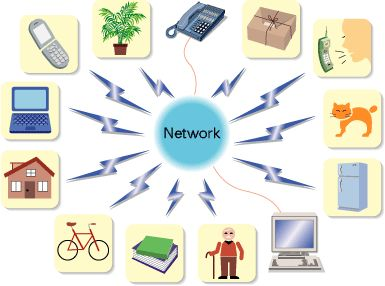
\includegraphics[scale=1.5]{figuras/ubiquitous.jpg}
    	\caption{Esquema de computação ubíqua}
	\label{esquema_computacao_ubiqua} 
    \end{figure}
\end{frame}

\begin{frame}
    \frametitle{SmartSpace}

    SmartSpaces são espaços onde a computação ubíqua acontece em sua totalidade.
    
    \begin{figure}[h]
    	\centering 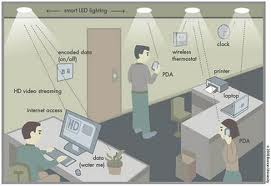
\includegraphics[scale=0.65]{figuras/smartSpace.jpg}
    	\caption{Smart Space}
    	\label{smart_space} 
    \end{figure}
\end{frame}

\begin{frame}
    \frametitle{Reconhecimento Facial}
    
    \begin{figure}[h]
	\centering 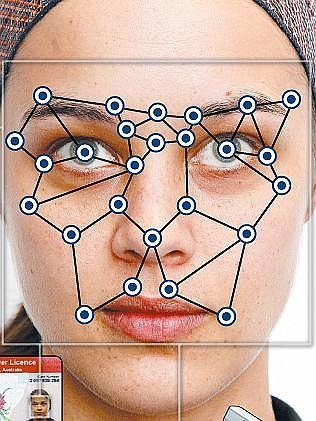
\includegraphics[scale=0.4]{figuras/face-recognition.jpg}
    	\caption{Exemplo de reconhecimento facial}
    	\label{reconhecimento_facial}
    \end{figure}-
\end{frame}

\begin{frame}
    \frametitle{Localização}
    \begin{figure}[h]
    \centering 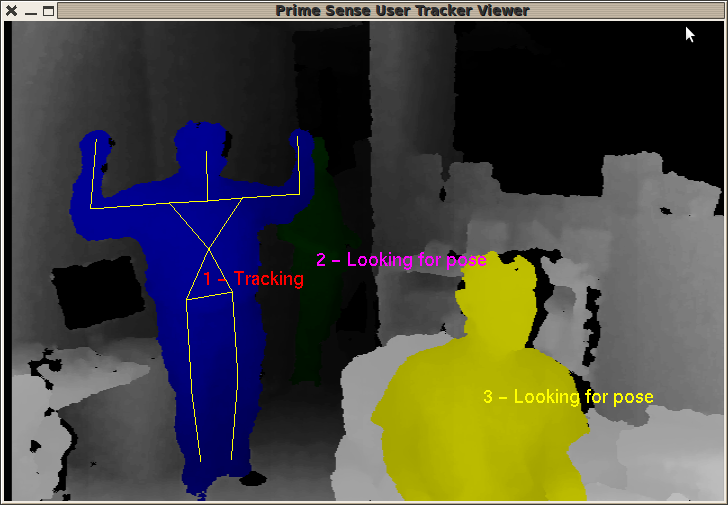
\includegraphics[scale=0.3]{figuras/sampleOpenNI.png}
        \caption{Rastreando os usuários presentes no ambiente}
        \label{sampleOpenNI}
    \end{figure}   
\end{frame}


\begin{frame}
    \frametitle{Kinect}
    
    \begin{figure}[h]
    \centering 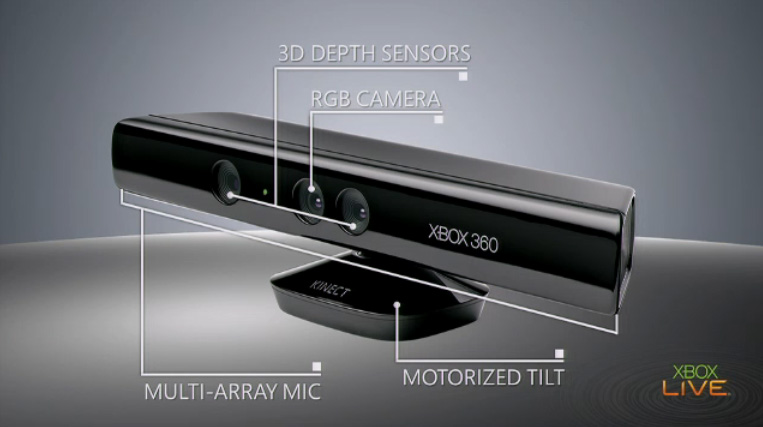
\includegraphics[scale=0.4]{figuras/kinect_info.jpg}
        \caption{Sensor Kinect da Microsoft utilizado no XBOX 360}
        \label{reconhecimento_facial}
    \end{figure}
\end{frame}

% ------------- Problema -------------
\section{Problema}
\begin{frame}
    \frametitle{Problema}
    \begin{itemize}
      \item Como fornecer para o \it{UnBiquitous} quem está presente no \it{SmartSpace} e onde este usuário está?
    \end{itemize}
\end{frame}

% ------------- Justificativa -------------
\section{Justificativa} 
\begin{frame}
    \frametitle{Justificativa}
    \begin{itemize}
      \item Para conseguir uma boa interação entre as diversas peças que compõem o SmartSpace é necessário que se tenha a disposição informações de contexto;
      \item Informações de contexto são importantes para definir ajustes finos nos componentes do ambiente;
      \item Para isso é necessária informações de contexto como:
	    \begin{itemize}
		\item Perfil
		\item Localização
	    \end{itemize}
    \end{itemize}
\end{frame}


% ------------- Sobre o trabalho -------------
\section{Sobre o Trabalho}
\begin{frame}
    \frametitle{Sobre o Trabalho}
    \begin{itemize}
        \item Como será executado?
        \item Qual a metodologia?
    \end{itemize}
\end{frame}

% ------------- Hipotese -------------
\subsection{Hipótese}
\begin{frame}
    \frametitle{Hipóteses}
    \begin{itemize}
      \item Que o sistema desenvolvido para o reconhecimento e localização de usuários em um SmartSpace seja robusto, confiável e rápido.
      \begin{itemize}
        \item Que \it{Eigenfaces}, método de reconhecimento facial que o \it{OpenCV} implementa, seja suficientemente confiável.
        \item Que o rastreamento fornecido pelo \it{OpenNI} seja suficientemente robusto para a dinâmicidade do ambiente.
      \end{itemize}
    \end{itemize}
\end{frame}

% ------------- Objetivos -------------
\subsection{Objetivos}
\begin{frame}
    \frametitle{Objetivos}
    \begin{itemize}
      \item \textbf{Objetivo Geral}
        \begin{itemize}
          \item Propor um sistema eficiente para reconhecimento e localização de usuários dentro de um SmartSpace em tempo real.
        \end{itemize}
      \item \textbf{Objetivo Específico}
        \begin{itemize}
            \item Implementar um sistema eficiente que através de imagens de cor e de profunidade providas pelo Kinect e utilizando as bibliotecas, \it{OpenCV} e \it{OpenNI}, reconheça os usuários e rastrei-o durante a sua permanência no \it{SmartSpace}.
        \end{itemize}
    \end{itemize}
\end{frame}

% ------------- Metodologia -------------
\subsection{Metodologia}
\begin{frame}
    \frametitle{Metodologia}
    \begin{itemize}
    \item Levantamento do estado da arte
        \begin{itemize}
            \item Identificação das limitações dos métodos utilizados e dos sensores (Kinect).
        \end{itemize}
    \pause \item Proposta de solução
    \pause \item Implementação.
    \pause \item Validar solução
        \begin{itemize}
            \item Em um ambiente bem delimitado e controlado, executar e avaliar a seu funcionamento e a sua eficiência em diferentes situações.
        \end{itemize}
    \end{itemize}
\end{frame}

% ------------- Resultados Esperados -------------
\subsection{Resultados Esperados}
\begin{frame}
    \frametitle{Resultados Esperados}
    \begin{itemize}
        \item Que o sistema proposto seja implementado e atinja o índice de confiança mínimo de 95\%.
    \end{itemize}
\end{frame}

% ------------- Cronograma -------------
\subsection{Cronograma}
\begin{frame}
    \frametitle{Cronograma}
    \begin{itemize}
        \item Julho: Levantamento do estado da arte
        \item Agosto: Implementação
        \item Setembro: Implementação, testes e documentação.
        \item Outubro: Término da implementação, documentação, conclusão da monografia, \textit{refactoring} e testes.
        \item Novembro: Análise de resultados, conclusão da monografia e preparação para apresentação
        \item Dezembro: Apresentação
    \end{itemize}
\end{frame}


% ------------- REFERENCIAS -------------

\nocite{fabriciobuzzeto,weiser2,saocarlos,yang,hewitt,violajones}

\section{Referências}

\frame[allowframebreaks]{
  \frametitle{Referências}
  \bibliographystyle{plain}
  \bibliography{bibliografia}
}

\begin{frame}
    \frametitle{ }
    \centerline{Obrigado!}
\end{frame}

\end{document}